\documentclass[tikz]{standalone}
\begin{document}
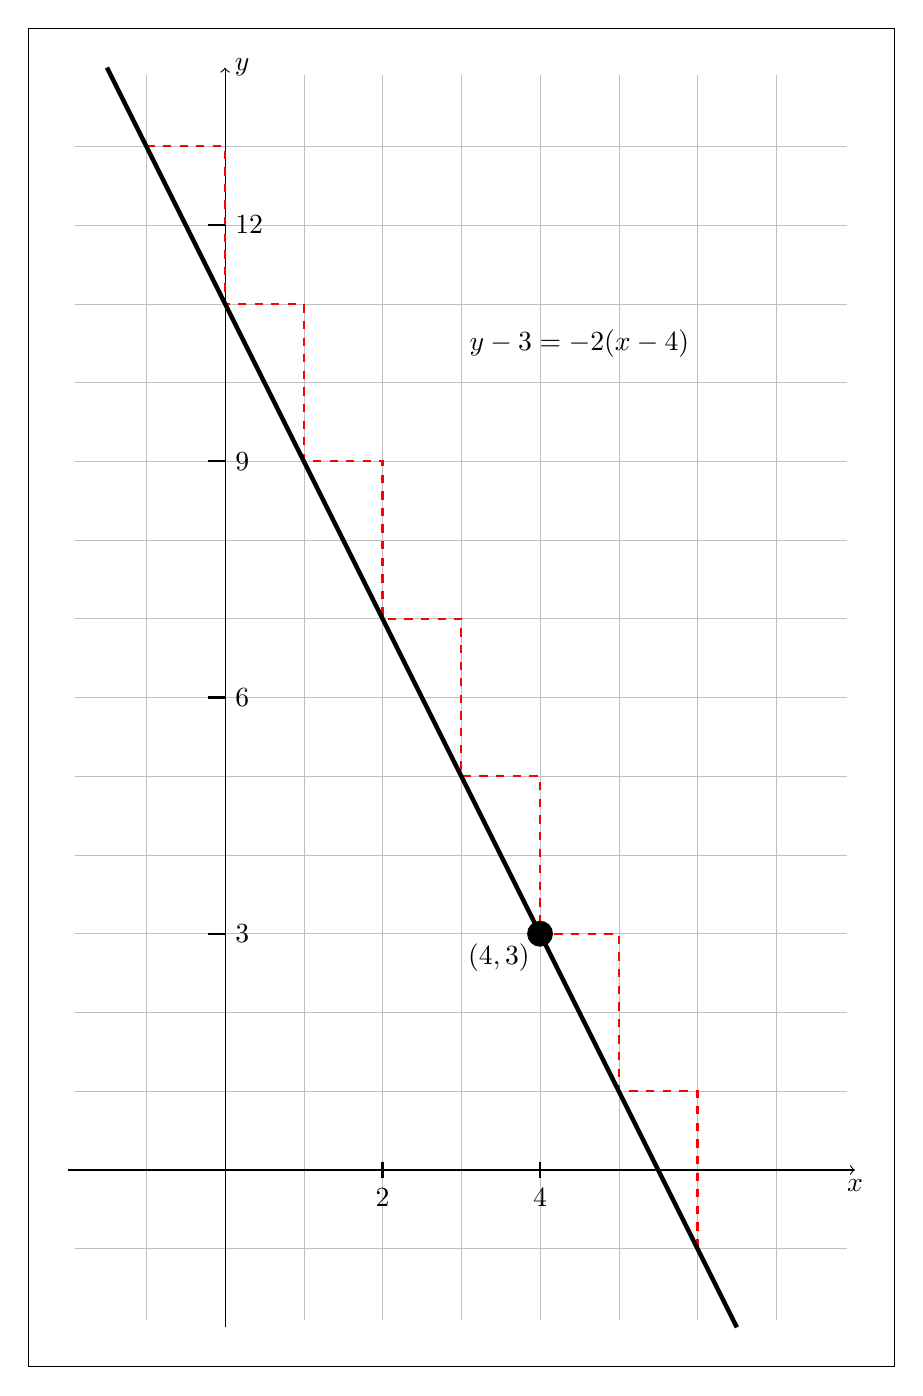
\begin{tikzpicture}[scale=1.0]
\draw[black,fill=white] (-2.5,-2.5) rectangle (8.5,14.5);
\draw[very thin,color=lightgray,step=1] (-1.9,-1.9) grid (7.9,13.9);
\draw[->] (-2,0) -- (8,0) node[below] {$x$};
\draw[->] (0,-2) -- (0,14) node[right] {$y$};
\node at (4.5, 10.5){$y - 3 = -2(x-4)$};

% draw slope
%\draw[dashed,red,thick] (-1,13)|- ++(1,-2) |- ++(1,-2) |- ++(1,-2) |- ++(1,-2) |- ++(1,-2) |- ++(1,-2) |- ++(1,-2);
\draw[dashed,red,thick] (-1,13) -| ++(1,-2) -| ++(1,-2) -| ++(1,-2) -| ++(1,-2) -| ++(1,-2) -| ++(1,-2) -| ++(1,-2);


% draw line and point
\draw[domain=-1.5:6.5,smooth,variable=\x,black,ultra thick] plot ({\x},{-2*\x + 11});
\draw [fill=black,thick] (4,3) circle [radius=0.15] node [below left] {$(4,3)$};

% tick marks
\foreach \x in {2,4} 
	\draw [thick] (\x cm,3pt) -- (\x cm,-3pt) node[below] {$\x$};
\foreach \y in {3,6,9,12} 
	\draw [thick] (-6pt,\y cm) -- (0pt,\y cm) node[right] {$\y$};
\end{tikzpicture}
\end{document}
